\documentclass[a4paper,12pt]{article}
\usepackage{fontawesome}
\usepackage{tabularx}
\usepackage{fullpage,graphicx,tikz}

%\usepackage{doublespace}
%\setstretch{1.2}

\usepackage{ae}
\usepackage{CV}
\usepackage{xcolor}
\usepackage{hyperref}
\hypersetup{
	colorlinks=true,
      linkcolor=blue,
    urlcolor=blue}

\begin{document}

\pagestyle{empty}

%Ueberschrift
\begin{center}
\huge{\textsc{Curriculum Vitae}}
\vspace{\baselineskip}

\end{center}
\vspace{1.5\baselineskip}
\begin{minipage}{0.7\textwidth}
\Large{\textsc{MD.Al-Helal}}\\
\end{minipage}
\begin{minipage}{0.7\textwidth}
  \begin{tikzpicture}
    \clip(0,0)circle[radius=1.37cm,];
    \node{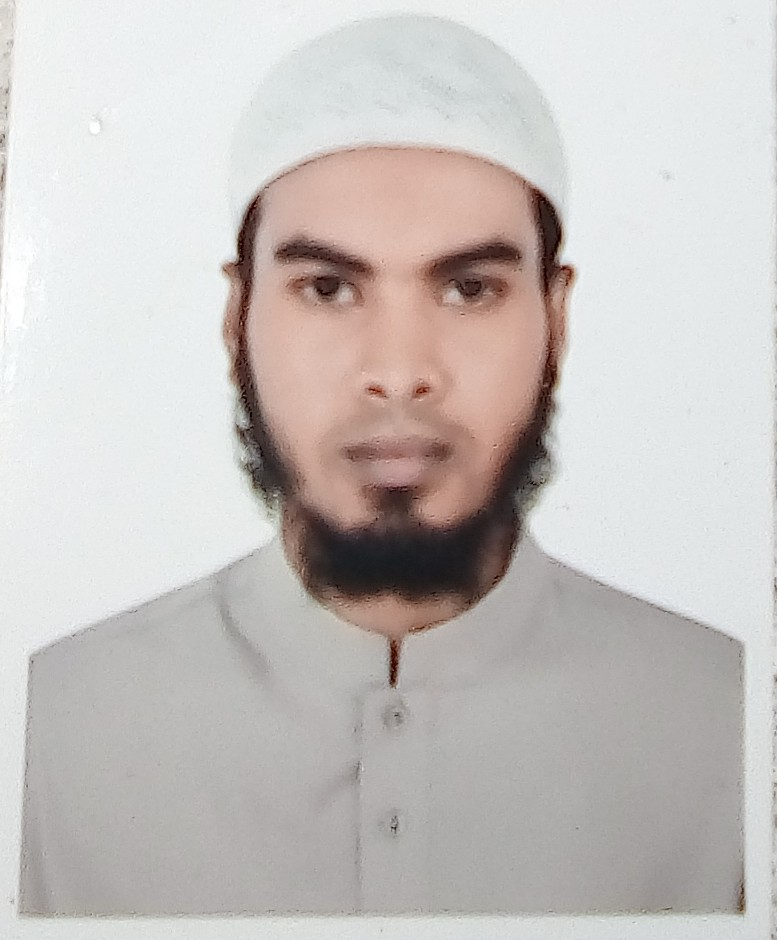
\includegraphics[scale=0.1]{Image/myPhoto.jpg}};   
\end{tikzpicture}
\end{minipage}
\section{Address}
\noindent
\begin{minipage}{.7\textwidth}
  Room no-1406\\
  Shahid Sarafat Ali Building\\
  Dr. Muhammad Shahidullah Hall\\
  University of Dhaka\\
  Dhaka-1000\\
\end{minipage}
\begin{minipage}{.7\textwidth}
  \faPhone{} 01515-611989\\
  \faEnvelopeO{}  \href{mailto:al2helal@gmail.com}{al2helal@gmail.com}\\
  \faGithub{}  \href{https://github.com/al2helal}{al2helal}\\
  \faLinkedin{}  \href{https://www.linkedin.com/in/mdalhelal/}{al2helal}\\
  \faStackOverflow{}  \href{https://stackoverflow.com/users/5697418/alhelal}{alhelal}
\end{minipage}

\section{Career Objective}
\begin{CV}
\item Solving real life problem those suffers humanity and making effective products for society by hard working and responsibility. And thereby build up an efficient career in the computer science and engineering and serve humanity.
  \end{CV}

\section{Job Experience}

\begin{CV}

\item[2019-2020] I performed as an assistant programmer at AIS ( Accounts and Information System ) Project, University of Dhaka from June 2019 to March 2020.
\end{CV}


\section{Education}

\begin{CV}
\item[2018] University of Dhaka, Dhaka-1000.\\Completed B.S in Computer Science \& Engineering.
\item[2014] Carmichael College, Rangpur.\\Passed H.S.C (Science Group) under Dinajpur Board in 2014.\\Obtained GPA 5.00 (without 4\textsuperscript{th} subject score) out of 5.00.
\item[2012] Moyenpur High School, Mithapukur, Rangpur.\\Passed S.S.C (Science Group) under Dinajpur Board in 2012.\\Obtained GPA 5.00 (without 4\textsuperscript{th} subject score) out of 5.00.
\end{CV}


%\section{Language Skills}
%\begin{table}[h] %\centering
%\begin{tabular}{p{2cm}>{}p{2.5cm}p{3cm}}
%Bangali  & native \\
%English  & 2nd language\\
%\end{tabular}
%\end{table}


%\section{Areas of Interest}
%\begin{CV}
%\item Machine learning, System programming, Making helpful shell script.
%\end{CV}


\section{Scholarship}

\begin{CV}
\item[2019] Obtained ICT fellowship for M.S thesis titled “Humanoid Robot Behavior Generation to Improve Social Skill of Autistic Children”.
\item[2009] Obtained National Education Board Scholarship for good result in class 8.
\item[2014] Obtained National Education Board Scholarship for good result in H.S.C under Dinajpur Board.
\end{CV}

%\section{Technical Skills}
%\begin{table}[h]
%  \begin{tabular}{p{5cm}>{}p{6cm}}
%    Programming Languages  & C, Java, Sql, Mysql, HTML, R, Assembly\\
%    Tools & Oracle database, PhpMyadmin\\
%Version Control  & Git\\
%IDE & IntelliJ, Netbeans, Code Blocks\\
%Text Editor & Vim\\
%Operating System & Ubuntu, Fedora, Windows\\
%Typesetting & \LaTeX{}, Open office, Microsoft office\\
%\end{tabular}
%\end{table}

\section{Technical Skills}

\begin{CV}
\item[Languages]  Java, PHP, Python, C, Sql, Mysql, HTML, CSS, JavaScript
\item[Tools] Oracle database, PhpMyadmin, AWS ( I had a server. I have some primary knowledge. )
\item[Framework] Django, Bootstrap
\item[VCS] Git
\item[IDE] IntelliJ, Netbeans, Code Blocks
\item[Text Editor] Vim, VSCode
\item[OS] Ubuntu, Fedora, Kali Linux, Windows
\item[Typesetting] \LaTeX{}, Open office, Microsoft office
\item[Typing Speed] 35 words/minute 
\end{CV}
\section{References}

\begin{table}[h]
\begin{tabular}{@{}lll@{}}
  \textbf{Dr. Saifuddin Md. Tareeq}\\
  Professor \& Chairperson\\
Computer Science \& Engineering\\
University of Dhaka\\
\faPhone{} 01715062737 ( Cell )\\
\faPhone{} 9661920-7430, 9670734-316 ( Office )\\
\faEnvelopeO{} \href{mailto:smtareeq@cse.du.ac.bd}{smtareeq@cse.du.ac.bd}\\
\end{tabular}
\end{table}

\noindent \today



\end{document}

%Tabellen
\begin{table}[htbp] \centering%
\begin{tabular}{lll}\hline\hline
1 & 2 & 3 \\ \hline
1 & \multicolumn{2}{c}{2} \\
\hline
\end{tabular}
\caption{Titel\label{Tabelle: Label}}
\end{table}
